\documentclass[twocolumn]{article}
\usepackage{bttda-paper}
\usepackage{todonotes}

\addbibresource{references.bib}
\addbibresource{moabb_datasets.bib}

\title{Block-Term Tensor Discriminant Analysis for Brain-Computer Interfacing}

\author{%
	A. Van Den Kerchove$^{1,2,*}$,
	H. Si-Mohammed$^{2}$,
	F. Cabestaing$^{2}$,
	M.M. Van Hulle$^{1}$
	\bigskip\\
	$^1$ KU Leuven,
	Leuven Brain Institute,
	Leuven.AI,\\
	Department of Neurosciences,
	Laboratory for Neuro- and Psychophysiology,
	\\
	Campus Gasthuisberg O\&N2,
	Herestraat 49 bus 1021,
	BE-3000 Leuven,
	Belgium
	\smallskip\\
	$^2$ Univ. Lille, CNRS, Centrale Lille,
	UMR 9189 CRIStAL,
	F-59000 Lille,
	France
	\smallskip\\
	$^*$ \texttt{arne.vandenkerchove@kuleuven.be}
}


\begin{document}

\maketitle

\begin{abstract}
	\input{abstract.txt}
\end{abstract}

\paragraph{Keywords}
\emph{%
	tensor discriminant analysis,
	brain-computer interface,
	block-term decomposition,
	multilinear decoding,
	event-related potentials,
	motor imagery
}

\section{Introduction}

\Acp{bci} have the potential to bypass
defective neural pathways by providing an alternative communication channel
between the brain and an external device.
These interfaces find applications in, among others, the development of neuroprosthetics and assistive
technologies~\cite{Wolpaw2020}.
To achieve their functionality, \acp{bci} record and process neural data obtained through
a neuroimaging technique, with \ac{eeg} being the most popular.

A \ac{bci} usually operates by identifying specific, task-related activity in
the recorded \ac{eeg} data, which can then be coupled to output or actions.
A well-known example is the P300 speller~\cite{Krusienski2006}.
Here, flashing stimuli representing characters evoke \acp{erp} that are recorded in the
\ac{eeg} signal.
The presence of the P300 component in this \ac{erp} encodes whether a given
stimulus was attended or not.
Decoding the stimulus that was attended can then be used to type the related
character.

Other paradigms, such as \ac{mi}~\cite{Aggarwal2019} instruct the user to imagine the movement of
one limb or the other.
The characteristic brain activity related to movement of the limb can be
detected from the \ac{eeg} signal in the form of event-related synchronization
and desynchronization and its corresponding spatial distribution,
which allows the \ac{bci} to measure for which limb a movement was
imagined.
The decoded category can then be used to control an assistive communication
device,
e.g.\ by selecting corresponding actions or moving a cursor.

In summary, these \ac{bci} problems give rise to classification problems (P300
\ac{erp} vs.\ non-attended \ac{erp}, left vs.\ right \ac{mi}, \ldots).
The decoding step occurs by applying a trained classifier to the  \ac{eeg}
data.
Due to the high inter-subject and inter-session variability encountered in
the \ac{eeg} signal, classifiers are often trained using a calibration period
at the beginning of the operation session.
To enhance the user experience, this calibration session should ideally have minimal
duration, resulting in small, subject- and session-specific training datasets.
This makes \ac{bci} classification methods vulnerable to overfitting in the
presence of high-dimensional data if no countermeasures are taken.
Hence, the dimensionality of the data must be reduced in a way that extracts as
many features containing information relevant to the classification problem as
possible, yet that is sparse enough to discard irrelevant features.

\subsection{Tensors \& tensor methods}

Due to its multichannel time series format, \ac{eeg} data, like most neural
signal acquisition modalities used for \acp{bci}, naturally exist as multiway data,
capturing information in both spatial and temporal domains.
Common preprocessing transformations, such as time-frequency transformation,
time-binning, or integrating information across multiple subjects or conditions,
can further expand the data into additional analytic domains.
This then results in high-dimensional datasets which are usually flattened into a
set of sample vectors, stripping the original data from its structure.
Yet, the intrinsic multiway structure of neural data~\cite{Erol2022} is
well-suited for representation as \emph{tensors}, or multiway arrays, where
each domain is represented as a tensor \emph{mode}.
Tensors provide a structured data representation for this highly dimensional
multiway data.
This in turn paves the way to the development of tensor methods which can
counteract some of the drawbacks of the dimensionality problem.
Tensor methods are machine learning techniques that consider each tensor mode
separately, reducing a given problem into partial, per-mode problems.

These tensor methods decompose a tensor into a lower dimensional structure of a
core tensor and factor tensors.
The most common approaches adhere to either the Tucker structure or the PARAFAC
structure.
A Tucker decomposition reduces an input tensor of size $(D_1,D_2,\ldots,D_K)$ to
a dense tensor of size $(R_1,R_2,\ldots,R_K)$ with $R_k \leq D_k$ using a
set of per-mode factor matrices.
Effective unsupervised tensor decomposition and approximation in the Tucker format can be achieved
using the \ac{hosvd}~\cite{DeLathauwer2000,SoleCasals2018}.
Alternatively, the PARAFAC structure can be used.
Here, the tensor is decomposed into a sum of rank-1 tensors, each the product
of a scalar and a vector per mode.
This is equivalent to a Tucker structured decomposition with all core elements
off the hyperdiagonal set to 0, as shown in \cref{fig:bttda/sparse}.
One way of obtaining an unsupervised PARAFAC decomposition is through the Canonical Polyadic
Decomposition~\cite{Hitchcock1927,Nazarpour2006}.
These decomposition methods can be regarded as feature extraction methods for a
\ac{bci} classification problem, with the flattened core tensors as feature vectors.
Extracted features can subsequently be further classified, most commonly
using \ac{lda} or a \ac{svm} to predict class labels.


\begin{figure*}[t]
	\centering
	\makebox[\linewidth][c]{%
		\bigskip
\footnotesize
\begin{tikzpicture}[x=\textwidth/14.2, y=-\textwidth/14.2]
  \TensorThree{data}{}{}{}{2}{2}{2}
  \begin{scope}[shift={((5.5,0)}]
    \TensorThree{core}{}{}{}{1}{1}{1}
	  \begin{scope}[shift={(-0.0707, -0.0707)}]
      \MatrixSkewed{fac. 1}{}{}{1}{1}
    \end{scope}
	  \begin{scope}[shift={(-0.1,0)}]
      \MatrixLeft{fac. 2}{}{}{1}{1}
    \end{scope}
	  \begin{scope}[shift={(0,1.1)}]
      \MatrixBelow{fac. 3}{}{}{1}{1}
    \end{scope}
  \end{scope}
  \begin{scope}[shift={(0,4)}]
      %\useasboundingbox (0,-1) rectangle (13,3.5);
      \TensorThree{$\ten{G}$}{}{}{}{2}{2}{2}
      \node[anchor=north, align=center] at (1,2) {Tucker structure};

      {\footnotesize
      \begin{scope}[shift={(5,0)}]
        \TensorThree{}{}{}{}{2}{2}{2}
        \node at (.33,.33,-.33) {$g^{(1)}$};
        \node at (.66,.66,-.66) {$g^{(2)}$};
        \node at (1,1,-1) {$\ddots$};
        \node at (1.5, 1.5, -1.5) {$g^{(b-1)}$};
        \node at (1.8, 1.9, -1.8) {$g^{(B)}$};
        %\node at (.25,.3,-.25) {$g^{(1)}$};
        %\node at (.75,.8,-.75) {$g^{(2)}$};
        %\node at (1.5,1.5,-1.5) {$\ddots$};
        %\node at (2.25,2.3,-2.25) {$g^{(B-1)}$};
        %\node at (2.75,2.8, -2.75) {$g^{(B)}$};

        %\TensorThree{$g^{(1)}$}{}{}{}{.5}{.5}{.5}
        %\node at (1.5,1.5,-1.5) {$\ddots$};
        %\begin{scope}[shift={(.5,.5,-.5)}]
        %  \TensorThree{$g^{(2)}$}{}{}{}{.5}{.5}{.5}
        %\end{scope}
        %\begin{scope}[shift={(2,2,-2)}]
        %  \TensorThree{$g^{(B-1)}$}{}{}{}{.5}{.5}{.5}
        %\end{scope}
        %\begin{scope}[shift={(2.5,2.5,-2.5)}]
        %  \TensorThree{$g^{(B)}$}{}{}{}{.5}{.5}{.5}
        %\end{scope}
      \end{scope}
      }
      \node[anchor=north, align=center] at (6,2) {PARAFAC structure};

      \begin{scope}[shift={(10,0)}]
        \TensorThree{}{}{}{}{2}{2}{2}
        \TensorThree{$\ten{G}^{(1)}$}{}{}{}{.5}{.5}{.5}
        \node at (.75,.75,-.75) {$\ddots$};
        \begin{scope}[shift={(1,1,-1)}]
        \TensorThree{$\ten{G}^{(B)}$}{}{}{}{1}{1}{1}
        \end{scope}
      \end{scope}
      \node[anchor=north, align=center] at (11,2) {block-term structure};
  \end{scope}
  \draw[->] (2,1, -1) -- (3.9,1,-1);
  \draw (6,2.5,-1) -| (6,3,-1);
  \draw[->] (6, 3,-1) -| (1,4,-1);
  \draw[->] (6, 3,-1) -| (6,4,-1);
  \draw[->] (6, 3,-1) -| (11,4,-1);
\end{tikzpicture}

	}
	\caption[Core tensor(s) of different tensor decomposition structures.]{%
		A tensor decomposition finds core tensor and factor matrices
		from input tensor.
		This core tensor can have several structures.
		In the Tucker structure, the core is a dense tensor $\ten{G}$.
		The PARAFAC structure expresses the core as a sum of $B$ rank-1 terms, each
		with a scalar core $g^{(b)}$.
		The block-term structure expresses the core as a sum of $B$ smaller,
		Tucker-structured blocks $\ten{G}^{(b)}$.
		Both the PARAFAC and block-term structures are more sparse than the full
		Tucker structure, yet the block-term structure is more flexible as it
		allows blocks of variable rank instead of scalars.

		%Core tensor(s) of different tensor decomposition structures.
		%The block-term and PARAFAC tensor decomposition
		%BTTDA and PARAFACDA can find a
		%sparser expression of the discriminant information captured by the dense,
		%Tucker-structured HODA algorithm.
	}\label{fig:bttda/sparse}%
\end{figure*}


While commonly used, these Tucker or PARAFAC structures might still not be able to
efficiently represent relevant neural information in a compressed format.
The block-term tensor structure is a generalization of the Tucker and
PARAFAC structures.
It represents the tensor as a sum of Tucker structured terms.
If the number of terms is equal to 1, it is equivalent to the Tucker structure; if the rank of each term is equal to 1, it is equivalent to the PARAFAC
structure.
The block-term structure is more flexible than either the Tucker or the PARAFAC
structures, since it is not constrained to solutions that must be expressed as
either one of these structures and their chosen hyperparameters.
Due to its flexibility, the block-term structure can strike a better
balance between extracting a maximal amount of relevant features and a minimal
amount of irrelevant features.
However, this increased flexibility comes at the cost of a higher number of
hyperparameters, as now both the number of terms and the multilinear rank of
each term need to be specified.
A block-term structured core tensor can be obtained in an unsupervised way using
the Block-Term Decomposition~\cite{DeLathauwer2008,DeLathauwer2008a,DeLathauwer2008b,Rontogiannis2021}.
Performance of methods leveraging either the Tucker and PARAFAC structures are
heavily dependent on the prior choice of hyperparameters describing
the multilinear rank or the number of rank-1 terms.
\subsection{Supervised tensor decompositions for \ac{bci}}

If the decompositions are not full rank, the Tucker, PARAFAC and block-term
structures are not unique and can be obtained by optimizing different criteria.
Given the low signal-to-noise ratio and specific, task-related output expected
in a BCI application, supervised feature extraction and machine learning techniques are
favored~\cite{Lotte2018} over the unsupervised decomposition methods presented
above.
A decomposition that is helpful for classification purposes should ideally optimize
the discriminability between classes in the resulting core tensors, which can
then be considered as extracted features.
In this philosophy, the Tucker decomposition can also be obtained
using \ac{hoda}~\cite{Yan2005,Phan2010,Froelich2018}, which optimizes class separability in the Fisher sense, analogous to linear
discriminant analysis.

Variants of \ac{hoda} have been applied to \ac{bci} problems such as
\ac{erp}~\cite{Onishi2012,Higashi2016} and \ac{mi}~\cite{Liu2015,Cai2021}
decoding with positive results~\cite{Lotte2018}.
Recent work proposes adaptations such as suited objective
functions and regularization~\cite{JamshidiIdaji2017,Jorajuria2022,Aghili2023}.
Discriminant tensor features have also been extracted
in the PARAFAC structure through manifold optimization~\cite{Froelich2018}.
However, it is not immediately obvious if either the Tucker or PARAFAC
structure are most suited to represent the neural data of interest for the
\ac{bci}
paradigm and for decoding.

More recent studies have shown that supervised decoders adopting a more flexible structure
can improve \ac{bci} performance.
Promising results have been achieved for regression tasks using
Higher Order Partial Least Squares~\cite{Camarrone2018} and Block-Term Tensor
Regression (BTTR)~\cite{Faes2022,Faes2022a}.
BTTR has also been adapted into a classification variant~\cite{Camarrone2021}
but this leaves room for improvement.
Instead of optimizing features directly for class separability, a dummy
independent variable was regressed towards, and the method
cannot be extended to a multi-class setting.
Furthermore, structures employed in these regression approaches are still more constrained
than what could be achieved with a full block-term tensor structured decomposition
optimized for discriminability, since they rely on a low-rank common subspace
between the input and classification labels.
\textcite{Huang2020} propose a supervised approach for finding multiple discriminant
multilinear spectral filter terms and apply it to motor imagery BCI, but their
decomposition is also restricted in flexibility, since the solution is
restricted to rank $(R_1,R_2,1)$ with mode 3 corresponding to the frequency domain.

\subsection{Contribution: A block-term structured model for classification}

A block-term decomposition that is directly optimized for discriminability and with a
proper choice of ranks and number of terms might better represent the behavior
of generators of neural activity through increased flexibility, or might
achieve better regularization through increased sparsity.
An alternative view on the same approach goes as follows:
If HODA with a well-chosen multilinear rank extracts some discriminant features
from the input tensor, it is likely that it does not yet retrieve all useful
information due to the restrictions imposed by its Tucker structure.
Could we therefore not keep using HODA to extract discriminant Tucker structured
terms as long as decoding performance increases?

We propose to implement this idea as a new supervised feature
extraction tensor method that is a generalization of the aforementioned
\ac{hoda}
algorithm and is more suited for the extraction of discriminant
features, while adhering to a flexible and efficient block-term tensor
structure.
This work features the following contributions:
\begin{enumerate*}[label={\arabic*)}]
	\item We develop a forward model for \ac{hoda} to reconstruct a
	      given input tensor from the extracted features.
	\item This allows us to introduce a state-of-the-art \ac{bci} feature extraction
	      method based on the block-term tensor structure, named \acf{bttda}.
	\item We evaluate a \ac{bci} decoder based on \ac{bttda} and its special
	      PARAFAC-structured case on decoding tasks for both \ac{erp} and \ac{mi}
	      paradigm \ac{bci} datasets.
\end{enumerate*}

\section{Methods}

\subsection{Notation}
Tensors are indicated by bold underlined letters $\ten{X}$, matrices by bold
letters $\mat{U}$, fixed scalars by uppercase letters $K$, and variable
scalars as lowercase letters $k$.
The $n^\text{th}$ sample of a tensor dataset with $N$ samples is written as
$\ten{X}(n)$, the dataset itself as ${\{\ten{X}(n)\}}_n^N$.
A tensor $\ten{X}\in \mathbb{R}^{D_1\times D_2 \times \cdots \times D_K}$ can be
unfolded in mode $k$ to a matrix
$\mat{X}_k\in\mathbb{R}^{(D_k\times\prod_{j\neq k}^K D_j)}$, by concatenating
all mode $j\neq k$ fibers.
The tensor-matrix product of tensor $\ten{X}$ with matrix $\mat{U}$ along a
given mode $k$ is written as $\ten{X}\mpr{\mat{U}}{k}$. For ease of notation, let
$\ten{X}\mmpr{\mat{U}} =
	\ten{X}\mpr{\mat{U}}{1}\mpr{\mat{U}}{2}\cdots\mpr{\mat{U}}{K}$.
When skipping one of the modes $k$, this is
written as $\ten{X}\mmprs{\mat{U}}{k} =
	\ten{X}\mpr{\mat{U}}{1}\mpr{\mat{U}}{2}\cdots\mpr{\mat{U}}{k-1}\mpr{\mat{U}}{k+1}\ldots\mpr{\mat{U}}{K}$.

\subsection{\Acl{hoda}}
\Acl{hoda}~\cite{Phan2010} is a
supervised tensor-based feature extraction technique.
For a set of $N$ tensors of order $K$
$\left\{\ten{X}(n)\in\mathbb{R}^{D_1\times D_2 \times \cdots \times
		D_K}\right\}_n^N$, HODA finds projection matrices $\mat{U_k}$ for each mode $k$
that project a given $\ten{X}$ to a latent tensor
$\ten{G}\in\mathbb{R}^{R_1\times R_2\times\cdots\times R_K}$, usually with lower
dimensionality $(R_1\leq D_1,R_2\leq D_2,\ldots,R_K\leq D_K)$ using
tensor-matrix mode products:
\begin{equation}
	\ten{G}  = \ten{X}\mmpr{\mat{U}}
	\label{eq:HODA-backward}
\end{equation}
as visualized in \cref{fig:HODA-backward}.
\begin{figure}[t]
	\centering
	\begin{tikzpicture}[y=-1cm]
	\TensorThree{$\ten{G}$}{$R_1$}{$R_2$}{$R_3$}{1}{1}{1}
	\node at (2,0.5) {$=$};
	\begin{scope}[shift={(4,0)}]
		\TensorThree{$\ten{X}$}{}{}{}{2}{2}{2}
		\begin{scope}[shift={(-0.0707, -0.0707)}]
			\MatrixSkewed{$\mat{U}_1$}{$D_1$}{$R_1$}{1}{2}
		\end{scope}
		\begin{scope}[shift={(-0.1,0)}]
			\MatrixLeft{$\mat{U}_2$}{$D_2$}{$R_2$}{1}{2}
		\end{scope}
		\begin{scope}[shift={(0,2.1)}]
			\MatrixBelow{$\mat{U}_3$}{$D_3$}{$R_3$}{2}{1}
		\end{scope}
	\end{scope}
\end{tikzpicture}

	\caption[A \acs{hoda} backward projection.]{%
		A visualization of the multilinear projection obtained by \acf{hoda} applied to a third-order tensor
		sample $\ten{X}$ with shape $(D_1,D_2, D_3)$.
		\Ac{hoda} finds projection matrices $\mat{U}_k$ such that maximal
		discriminability between classes is achieved in the projected latent tensors
		$\ten{G}$ with reduced dimensionality $(R_1,R_2,R_3)$.}
	\label{fig:HODA-backward}%
\end{figure}

Analogous to the \ac{hosvd}, \ac{hoda} is a dimensionality
reduction decomposition that results in a dense latent tensor $\ten{G}$, and
imposes an orthogonality constraint on $\mat{U}_k$ to ensure uniqueness.
However, while for the \ac{hosvd} decomposition the projection matrices
are chosen to minimize the reconstruction error, the projection matrices
$\mat{U}_k$ of \ac{hoda} are optimized for maximal discriminability of tensors
$\ten{G}(n)$ belonging to classes with labels $c_n$.
This is a desirable property in a classification setting where samples are
high-dimensional tensors.

\Ac{hoda} optimizes discriminability in the Fisher sense, by optimizing the
Fisher ratio $\phi$ between the latent tensors $\ten{G}(n)$:
\begin{equation}
	\phi = \frac{\sum_c^CN_c\left\|\bar{\ten{G}}(c)-\bar{\bar{\ten{G}}}\right\|_F^2}
	{\sum_n^N\left\|\ten{G}(n)-\bar{\ten{G}}(c_n)\right\|_F^2}
	\label{eq:fisher}
\end{equation}
for $C$ classes with each $N_c$ samples. $\bar{\ten{G}}(c)$ is the mean of
latent tensors of class $c$, and $\bar{\bar{\ten{G}}}$ the mean of
these class mean latent tensors.
If the ranks $(R_1,R_2, \ldots,R_k)$ are set a priori, the goal is now to find the optimal projection matrices:
\begin{equation}
	\left\{\mat{U}^*\right\} = \argmax_{\{\mat{U}\}}\phi
\end{equation}
which is solved through the HODA algorithm.
To start, $\mat{U}_k$ are initialized to orthogonal matrices, e.g.\ as random
orthonormal matrices, by a per-mode Singular Value Decomposition (SVD),
or as the partial \ac{hosvd} of all stacked tensors in the dataset.
At each iteration, the algorithm loops through the modes and fixes all
projections but $\mat{U}_k$ corresponding to mode $k$.
It then finds a partial latent tensor:
\begin{equation}
	\ten{G}_{-k}=\ten{X}\mmprs{\mat{U}}{k}
\end{equation}
Subsequently, a new projection matrix $\mat{V}_k$ can be found analogous to Linear
Discriminant Analysis by constructing the within-class scatter matrix:
\begin{equation}
	\mat{S}_{-k,\text{w}} = \sum_n^N\tilde{\mat{G}}_{-k,k}(n)\cdot\tilde{\mat{G}}_{-k,k}^\intercal(n)
\end{equation}
with $\tilde{\ten{G}}_{-k}(n) = \ten{G}_{-k}(n) - \bar{\ten{G}}_{-k}(c_n)$,
and the between-class scatter matrix:
\begin{equation}
	\mat{S}_{-k,\text{b}} =
	\sum_c^CN_c\tilde{\bar{\mat{G}}}_{-k,k}(c)\cdot\tilde{\bar{\mat{G}}}_{-k,k}^\intercal(c)
\end{equation}
with $\tilde{\bar{\ten{G}}}_{-k}(c) = \bar{\ten{G}}_{-k}(c) - \bar{\bar{\ten{G}}}_{-k}$,
and solving for the $r_k$ leading eigenvectors in the eigenvalue problem:
\begin{equation}
	\mat{S}_{-k,\text{b}}-\varphi_k\mat{S}_{-k,\text{w}} =
	\mat{V}_k\mat{\Lambda}\mat{V}_k^\intercal
\end{equation}
with $\varphi_k=\tr\left(\mat{U}_k^\intercal\mat{S}_{-k,\text{b}}\mat{U}_k\right)/\tr\left(\mat{U}_k^\intercal\mat{S}_{-k,\text{w}}\mat{U}_k\right)$
using the $\mat{U}_k$ obtained in the previous iteration.
Finally, the orthogonal transformation invariant projections $\mat{U}_k$
are obtained by calculating the
per-mode total scatter matrices:
\begin{equation}
	\mat{S}_{k,\text{t}} = \sum_n^N\mat{X}_k(n)\cdot\mat{X}_k^\intercal(n)
\end{equation}
and finding the $r_k$ leading eigenvectors of:
\begin{equation}
	\mat{V}_k\mat{V}_k^\intercal\mat{S}_{k,\text{t}}\mat{V}_k\mat{V}_k^\intercal
	= \mat{U}_k\mat{\Lambda}\mat{U}_k^\intercal
\end{equation}
at each iteration~\cite{Wang2007}.
The iterative process halts after a fixed number of iterations, or when the
update of each $\mat{U}_k$ is lower than a predetermined threshold.
The full \ac{hoda} procedure is summarized in \cref{alg:HODA}.
\begin{algorithm}
	\caption[A \acs{hoda} backward solution.]{The \acs{hoda} backward solution.}
	\label{alg:HODA}
	\begin{algorithmic}[1]
	\Require $\{\ten{X}(n)\}_n^N$, $\{c_n\}_n^N$,
	$(R_1,R_2,\ldots,R_K)$, $I_\text{max}$, $\epsilon$
	\State $\mat{U}_k \gets $ orthonormal matrix $\in \mathbb{R}^{D_k\times R_k}
		\ \forall k$
	\State $\mat{S}_{k,\text{t}} \gets
		\textstyle{\sum_n^N}\mat{X}_k(n)\cdot\mat{X}_k^\intercal(n)\ \forall k$
	\State $i\gets 1$
	\Repeat
	\For{$k=1,2\ldots,K$}
	\State $\ten{G}(n)_{-k} \gets \ten{X}(n)\mmprs{\mat{U}}{k} \ \forall n$
	\State $\mat{S}_{-k,\text{w}} \gets
		\textstyle{\sum_n^N}\tilde{\mat{G}}_{-k,k}(n)\cdot\tilde{\mat{G}}_{-k,k}^\intercal(n)$
	\State $\mat{S}_{-k,\text{b}} \gets
		\textstyle{\sum_c^C}N_c\tilde{\bar{\mat{G}}}_{-k,k}(c)\cdot\tilde{\bar{\mat{G}}}_{-k,k}^\intercal(c)$
	\State $\varphi_k\gets\tr\left(\mat{U}_k^\intercal \mat{S}_{-k,\text{b}}\mat{U}_k\right)/\tr\left(\mat{U}_k^\intercal\mat{S}_{-k\text{w}}\mat{U}_k\right)$
	\State $\mat{V}_k\gets$ \parbox[t]{5cm}{largest magnitude $R_k$ \\ eigenvectors of
	$\mat{S}_{-k,\text{b}} - \varphi_k\mat{S}_{-k,\text{w}}$}
	\State $\mat{U}_k \gets$ \parbox[t]{5cm}{largest magnitude $R_k$ \\
	eigenvectors of $\mat{V}_k\mat{V}_k^\intercal\mat{S}_{k,\text{t}}\mat{V}_k\mat{V}_k^\intercal$}
	\EndFor
	\State $i\gets i+1$
	\Until{$i=I_\text{max}$ or $||\mat{U}_k^{(i)}-\mat{U}_k^{(i-1)}||<\epsilon
		\ \forall k$}
\end{algorithmic}

\end{algorithm}

To apply \ac{hoda} in a classification setting, the projections
are first learned on a training dataset with known class labels.
Next, these projections are used to extract latent tensors from the
tensors in the training dataset.
These latent training tensors are then reshaped (\emph{vectorized}) into feature vectors
$\mat{g} =  \vect(\ten{G})$ and used to train a decision classifier with the corresponding class labels.
At the evaluation stage, the projections learned from the training dataset are
used to extract latent tensors from an unseen test dataset with unknown class
labels, which can also be vectorized and passed on to the trained decision
classifier.

To avoid overfitting and improve performance in low sample size settings, the
HODA problem can be regularized by shrinking the partial
within-class scatter matrices~\cite{Phan2010} with a shrinkage factor
$\alpha_k$ at each step such that the eigenvalue problem becomes:
\begin{equation}
	\mat{S}_b^{(-k)} -
	\varphi\left[\left(1-\alpha_k\right)\mat{S}_{-k,\text{w}}+\alpha_k\mat{I}\right] =
	\mat{V}_k\mat{\Lambda}\mat{V}_k^\intercal
\end{equation}
As in Linear Discriminant Analysis, the shrinkage parameter $\alpha_k$ can
also be estimated in a data-driven way in HODA~\cite{Jorajuria2022},
e.g., using the Ledoit-Wolf procedure~\cite{Ledoit2003} at every iteration.

\subsection{A forward model for \acs{hoda}}
As a prerequisite to the proposed \ac{bttda} model, we must find a
way to reconstruct the original data tensor $\ten{X}$ as accurately as possible
from $\ten{G}$ after dimensionality reduction.
This is usually referred to as finding a corresponding \emph{forward model}.
While a \emph{backward model} extracts latent sources or properties from the observed
data based on some task-related criterion or on prior domain knowledge,
a \emph{forward} model is a generative model that expresses the observed data in
terms of these latent properties or sources that are given.
Forward models are useful for, among other things, interpretability and data compression.

The \ac{hoda} projection in \cref{eq:HODA-backward} is an example
of a backward model.
A straightforward and computationally efficient candidate for a corresponding
forward model, visualized in \cref{fig:HODA-forward}, is given by:
\begin{equation}
	\ten{X} = \ten{G}\mmpr{\mat{A}^\intercal} + \ten{E} =
	\hat{\ten{X}} + \ten{E}
	\label{eq:HODA-forward}
\end{equation}
with \emph{activation patterns} $\mat{A}_k \in \mathbb{R}^{D_k\times R_k}$,
reconstructed tensor $\hat{\ten{X}}$, and error term $\ten{E}$.
\begin{figure*}[t]
	\centering
	\footnotesize
\begin{tikzpicture}[y=-1cm]
	\TensorThree{$\ten{X}$}{$D_1$}{$D_2$}{$D_3$}{2}{2}{2}
	\node at (3.25,.5){$=$};

	\begin{scope}[shift={(6.25,0)}]
		\begin{scope}[shift={(-0.0707, -0.0707)}]
			\MatrixSkewed{$\mat{A}_1$}{$R_1$}{$D_1$}{2}{1}
		\end{scope}
		\begin{scope}[shift={(-0.1,0)}]
			\MatrixLeft{$\mat{A}_2$}{$R_2$}{$D_2$}{2}{1}
		\end{scope}
		\begin{scope}[shift={(0,1.1)}]
			\MatrixBelow{$\mat{A}_3$}{$R_3$}{$D_3$}{1}{2}
		\end{scope}
		\TensorThree{$\ten{G}$}{}{}{}{1}{1}{1}

		\node at (1.75,.5){$+$};

		\begin{scope}[shift={(2.25,0)}]
			\TensorThree{$\ten{E}$}{}{}{}{2}{2}{2}
		\end{scope}


	\end{scope}



\end{tikzpicture}

	\caption[A forward projection for \ac{hoda}.]{The forward projection for HODA.
		By calculating activation patterns $\mat{A}_k$, the original tensor $\ten{X}$ can approximately be
		reconstructed from projected latent tensor $\ten{G}$.
		The reconstruction is accurate up to an error term $\ten{E}$.
		$\mat{A}_k$ are chosen such that the variability captured in the latent tensor is
		maximally expressed in the reconstructed tensor $\hat{\ten{X}}$ and not in
		the error term $\ten{E}$.}
	\label{fig:HODA-forward}
\end{figure*}

A good forward model should ensure that the norm of the reconstruction error
$\left\|\ten{E}\right\|_F$ is minimized.
In other words, variation captured in the latent tensor should be maximally captured by the
reconstruction term $\hat{\ten{X}}= \ten{G}\mmpr{\mat{A}^\intercal}$, and not by the error term
$\ten{E}$~\cite{Haufe2014}.
Hence, we aim to minimize the expected value of the cross-covariance between
the noise term and the extracted latent tensors:
\begin{equation}
	\left\{\mat{A}^*\right\}
	= \argmin_{\{\mat{A}\}}\text{E}\left[
		\text{vec}\left(\ten{E}(n)\right)\text{vec}\left(\ten{G}(n)\right)
		\right]_n
\end{equation}
or, equivalently~\cite{Parra2005,Haufe2014},
\begin{align}
	\left\{\mat{A}^*\right\}
	 & = \argmin_{\{\mat{A}\}}\sum_n^N\left[\ten{X}(n) -
	\hat{\ten{X}}(n)\right]^2                                                              \\
	 & = \argmin_{\{\mat{A}\}}\sum_n^N\left[\ten{X}(n) - \ten{G}(n)\mmpr{\mat{A}}\right]^2
\end{align}
This least-squares tensor approximation problem can be solved efficiently using the
alternating least squares algorithm~\cite{Bentbib2022}, iteratively fixing all but one of the activation patterns such that:
\begin{equation}
	\mat{A}_k = \argmin_{\mat{A}_k}
	\sum_n^N\left[\mat{X}_k(n) -
		\mat{A}_k\left(\ten{G}(n)\mmprs{\mat{A}}{k}\right)_k\right]^2
\end{equation}
at every iteration, which can be solved directly using ordinary least squares.
The activation patterns are initialized to the weights $\{\mat{U}\}$ of the
backward model.
Similar to fitting the backward model, the iterative process for the forward
model halts after a fixed number of iterations or when the update of each
$\mat{A}_k$ is lower than a predetermined threshold.
The full algorithm to determine the HODA forward projection is listed
in \cref{alg:HODA-fw}.
\begin{algorithm}
	\caption[A \acs{hoda} forward solution.]{The \acs{hoda} forward solution.}
	\label{alg:HODA-fw}
	\begin{algorithmic}[1]
	\Require $\{\ten{G}(n)\}_n^N,\{\ten{X}(n)\}_n^N,I_\text{max}, \epsilon$
	\State $\mat{A}_k \gets $ $\mat{U}_k \ \forall k$
	\State $i\gets 1$
	\Repeat
	\For{$k=1,2\ldots,K$}
	\State $\mat{X}_{-k}(n)\gets\ten{G}(n)\mmprsi{\mat{A}}{k} \ \forall n$
	\State
	$\mat{A}_k\gets\textstyle{\argmin_{\mat{A}_k}\sum_n^N}\left[\mat{X}_k(n)-\mat{A}_k\mat{X}_{-k}(n)\right]^2$
	\EndFor
	\State $i\gets i+1$
	\Until{$i=I_\text{max}$ or $||\mat{A}_k^{(i)}-\mat{A}_k^{(i-1)}||<\epsilon\
		\forall k$}
\end{algorithmic}

\end{algorithm}

The forward model could alternatively be specified in the classical manner by linear
regression or with the solution of \textcite{Haufe2014}, but this would require
vectorizing the tensor representation.
While the reconstruction error might be reduced, we would lose the computational
efficiency and regularizing constraints of the tensor form.
More efficiently, the forward model could be obtained through other tensor
regression methods, like Higher Order Partial
Least Squares.
This method still requires fitting more parameters than our
proposed model, on top of additional hyperparameters defining the
dimensionality of the common subspace.
An attractive property of our multilinear forward model for HODA is that it
estimates exactly as many parameters as the backward model, with the intuition that
it should not disproportionally contribute to overfitting.

\subsection{\Acl{bttda}}
After defining the forward model, we can construct our proposed block-term
tensor model.
Assuming the latent tensors $\ten{G}$
obtained by the backward projection of HODA do not achieve perfect
class separation, the error term $\ten{E}$ in
\cref{eq:HODA-forward} should still contain some discriminative
information, which can be exploited to improve classifier
performance.
Useful features can still be extracted from $\ten{E} = \ten{X} -
	\hat{\ten{X}}$, so it is further projected onto another core tensor
$\ten{G}^{(2)}$ (assuming $\ten{G}$ as $\ten{G}^{(1)}).$

We thus extend the \ac{hoda} feature extraction scheme to \acf{bttda}.
\Ac{bttda} finds multiple discriminative blocks, such that its forward
model adheres to the block-term tensor structure:
\begin{equation}
	\ten{X} = \sum_b^B\ten{G}^{(b)}\mmpr{\mat{A}^{(b)}} + \ten{E}
	\label{eq:BTTDA-forward}
\end{equation}
for $B$ extracted latent tensors $\ten{G}^{(b)}$ and residual error term
$\ten{E}$.
The BTTDA model is further illustrated by~\cref{fig:BTTDA}.
\begin{figure*}[t]
	\centering
	\footnotesize
\begin{tikzpicture}[y=-1cm]
	\useasboundingbox (0,-2) rectangle (16.5,3.5);
	\TensorThree{$\ten{X}$}{$D_1$}{$D_2$}{$D_3$}{2}{2}{2}

	\node at (3.15,0.5,0) {$=$};

	\begin{scope}[shift={(6.2,0)}]
		\begin{scope}[shift={(-0.0707, -0.0707)}]
			\MatrixSkewed{$\mat{A}_1^{(1)}$}{$R_1^{(1)}$}{$D_1$}{2}{1}
		\end{scope}
		\begin{scope}[shift={(-0.1,0)}]
			\MatrixLeft{$\mat{A}_2^{(1)}$}{$R_2^{(1)}$}{$D_2$}{2}{1}
		\end{scope}
		\begin{scope}[shift={(0,1.1)}]
			\MatrixBelow{$\mat{A}_3^{(1)}$}{$R_3^{(1)}$}{$D_3$}{1}{2}
		\end{scope}
		\TensorThree{$\ten{G}^{(1)}$}{}{}{}{1}{1}{1}
	\end{scope}

	\node at (8.30,0.5,0) {$+\cdots+$};

	\begin{scope}[shift={(11.85,0)}]
		\begin{scope}[shift={(-0.0707, -0.0707)}]
			\MatrixSkewed{$\mat{A}_1^{(B)}$}{$R_1^{(B)}$}{$D_1$}{2}{1}
		\end{scope}
		\begin{scope}[shift={(-0.1,0)}]
			\MatrixLeft{$\mat{A}_2^{(B)}$}{$R_2^{(B)}$}{$D_2$}{2}{1}
		\end{scope}
		\begin{scope}[shift={(0,1.1)}]
			\MatrixBelow{$\mat{A}_3^{(B)}$}{$R_3^{(B)}$}{$D_3$}{1}{2}
		\end{scope}
		\TensorThree{$\ten{G}^{(B)}$}{}{}{}{1}{1}{1}
	\end{scope}

	\node at (13.6,0.5,0) {$+$};

	\begin{scope}[shift={(14,0)}]
		\TensorThree{$\ten{E}^{(B)}$}{}{}{}{2}{2}{2}
	\end{scope}

\end{tikzpicture}

	\caption[A forward model for \acs{bttda}.]{A forward model for \acf{bttda}.
		\Ac{bttda} can extract more features
		than \ac{hoda} by iteratively finding a latent tensor $\ten{G}^{(b)}$ in a
		deflation scheme.
		The \ac{hoda} backward projection is first applied. Next, the
		input data is reconstructed via the HODA forward model and the
		difference between the two is found.
		Finally, this process is repeated with this difference as input data, until a
		desired number of blocks $B$ has been found.}
	\label{fig:BTTDA}
\end{figure*}
The block-term structure of this model implies that it is a generalization of both
the Tucker-structured \ac{hoda} and PARAFAC-structured discriminant feature
extraction.
If $B$ in \cref{eq:BTTDA-forward} is set to one, \ac{bttda} is equivalent to
\ac{hoda}; if at each term $b$ the rank of the core tensor
$(R_1^{(b)}=R_2^{(b)}=\ldots=R_k^{(b)}=1)$, a PARAFAC structure is assumed and
the resulting discriminant model is denoted as \ac{parafacda}.

Since \ac{bttda} is specified above as a forward model, a backward procedure
is required which finds the latent tensors $\ten{G}^{(b)}$ given $\ten{X}$ for
\ac{bttda} to be useful as a feature extraction method.
The extracted features represented by the latent tensors $\ten{G}^{(b)}$ can be
computed through a deflation scheme summarized in \cref{alg:BTTDA}.
\begin{algorithm}
	\caption[A \acs{bttda} feature extraction.]{\Ac{bttda}.}
	\label{alg:BTTDA}
	\begin{algorithmic}[1]
	\Require $\{\ten{X}(n)\}_n^N$, $\{c_n\}_n^N$,
	$\{(R_1^{(b)},R_2^{(b)},\ldots,R_K^{(b)})\}_b^B$
	\State $\ten{E}(n)\gets\ten{X}(n)\ \forall n$
	\For{$b=1,2,\ldots,B$}
	\State $\{\mat{U}^{(b)}\}\gets$ \parbox[t]{5cm}{\textsc{hoda} on $\{\ten{E}(n)\}_n^N$ and
	$\{c_n\}_n^N$ with rank $(R_1^{(b)},R_2^{(b)},\ldots,R_K^{(b)})$}
	\State $\ten{G}^{(b)}(n)\gets\ten{E}(n)\mmpri{\mat{U}^{(b)}}\
		\forall n$
	\State $\{\mat{A}^{(b)}\}\gets$ \parbox[t]{5cm}{Forward \textsc{hoda} on
		$\{\ten{G}^{(b)}(n)\}_n^N$ and $\ten{E}$}
	\State
	$\hat{\ten{E}}(n)\gets\ten{G}^{(b)}(n)\mmpri{\mat{A}^{\intercal(b)}}\
		\forall n$
	\State
	$\ten{E}(n)\gets \ten{E}(n) - \hat{\ten{E}}(n) \forall n$

	\EndFor
\end{algorithmic}

\end{algorithm}
For each block $b$, the latent tensor is extracted using the HODA backward
projection in \cref{eq:HODA-backward} from the residual error term of the previous
block $\ten{E}^{(b-1)}$:
\begin{equation}
	\ten{G}^{(b)} = \ten{E}^{(b-1)}\mmpr{\mat{U}^{(b)}}
\end{equation}
This residual error term is calculated by finding the difference between the
previous error and its reconstruction after backward and forward \ac{hoda}
projection:
\begin{align}
	\ten{E}^{(b)}
	 & = \ten{E}^{(b-1)} - \hat{\ten{E}}^{(b-1)}                      \\
	 & = \ten{E}^{(b-1)} - \ten{G}^{(b)}\mmpr{\mat{A}^{\intercal(b)}}
\end{align}
with $\ten{E}^{(0)}=\ten{X}$.

The resulting latent tensors can be vectorized and concatenated into
one single feature vector per input tensor:
\begin{equation}
	\mat{g}
	=\left[\vect\left(\ten{G}^{(1)}\right)\
		\vect\left(\ten{G}^{(2)}\right)\
		\cdots\
		\vect\left(\ten{G}^{(B)}\right)\right]
\end{equation}
so that they can be classified in a similar manner to HODA.


\subsection{Model and feature selection}
Similar to the unsupervised Block-Term Decomposition, the performance of
\ac{bttda} is
heavily dependent on the number of blocks $B$ and their corresponding ranks
$\left\{\left(R_1^{(b)}, R_2^{(b)}, \ldots,
	R_K^{(b)}\right)\right\}_b^B$.
If these are not known a priori, i.e., if they cannot be set based on insights into the
data generation process, a model selection step is necessary in order to
determine the optimal values for $R_k^{(b)}$ and $B$.
These hyperparameters can be set through cross-validated hyperparameter tuning,
but this can be a computationally expensive process.

To simplify the hyperparameter search and reduce the search space, we introduce
a single hyperparameter $\theta \in [0,1]$ which replaces the block ranks
$\left\{\left(R_1^{(b)}, R_2^{(b)}, \ldots,	R_K^{(b)}\right)\right\}_b^B$.
The new hyperparameter $\theta$ then controls the sparsity of the \ac{bttda} solution, with $\theta=0$
corresponding to the \ac{parafacda} model with blocks of rank 1, and $\theta=1$
corresponding to blocks of full rank $(D_1, D_2,\ldots,D_K)$.
For $0 < \theta < 1$, the multilinear rank of block $b$ can be determined
analogous to the method described by \textcite{Phan2010}.
Here, $R_k$ are chosen based on the number of components needed to explain a
certain proportion of the variability in a mode of the input data for a
Tucker-structured decomposition.
In our \ac{bttda} model, this can be achieved using the eigenvalues of the per-mode total scatter matrix of block input tensor $\ten{E}^{(b-1)}$
\begin{equation}
	\mat{S}_{k,\text{t}}^{(b)} = \sum_n^N\mat{E}_k^{(b-1)}(n)\cdot\mat{E}_k^{(b-1)\intercal}(n)
	= \mat{W}_k^{(b)}\mat{\Lambda}_k^{(b)}\mat{W}_k^{(b)\intercal}
\end{equation}
such that
\begin{equation}
	R_k^{(b)} = \argmin_{R\in 1,\ldots,D_k}\frac{\sum_r^R\lambda_{k,r}^{(b)}}{\sum_r^{D_k}\lambda_{k,r}^{(b)}} > \theta
\end{equation}

Finally, \ac{hoda}, and by extension \ac{bttda}, can extract a substantial amount
of redundant features, which can be dropped after projection and before proceeding to the classification
step~\cite{Phan2010}.
Specifically, in \ac{bttda} redundant features can accumulate over the number of
blocks, hampering performance.
Relevant features can be retained by calculating the
univariate Fisher score for all features.
The Fisher score $\phi(i)$ for feature $i$ is obtained as:
\begin{equation}
	\phi(i) = \frac
	{\sum_c^C N_c \left(\bar{g}_i(c)-\bar{\bar{g}}_i\right)^2}
	{\sum_n^N \left(g_i(n)-\bar{g}_i(c_n)\right)^2}
\end{equation}
The features can then either be sorted by $\phi(i)$, and a given number of
features retained for classification, or the decision to retain a feature can
be made by a threshold on the statistical $p$-value corresponding to the
$\phi(i)$.
We opted for the latter strategy since it avoids tuning an additional
hyperparameter.

\section{Experiments}
\subsection{Datasets and decoders}
We evaluated our proposed model in two offline EEG-based BCI decoding problems:
the event-related potential (ERP) and motor imagery (MI) paradigms using a
the openly available MOABB benchmarking datasets (version 1.2.0)~\cite{Aristimunha2023}.
Details about these datasets are found in \cref{tab:moabb}.
For the ERP datasets, the task is to distinguish target from non-target ERPs,
while the MI datasets consist of distinguishing different imagined limb
movements.
Within-session classification performance was assessed using stratified 5-fold
cross-validation to calculate the area under the receiver operating
characteristic curve (ROC-AUC) for binary classification problems and accuracy
for multi-class problems, as established by the benchmarking framework laid out
by \textcite{Aristimunha2023}.

To use HODA, BTTDA and PARAFACDA as a decoders, they are paired with LDA to classify the
extracted feature (HODA+LDA).
Hyperparameters $\theta$ in the case of HODA and BTTDA, and$B \in
	\left\{1,2\ldots,16\right\}$ in the case of were tuned separately for each
evaluation fold using nested, stratified 5-fold cross-validation.
Other HODA hyperparameters were set to $\varepsilon=\num{1e-8}$ and $I_\text{max}=128$.

Furthermore, as additional comparison methods, we used the methods evaluated by
\textcite{Chevallier2024}.
For the ERP datasets, these were the Riemannian Geometry-based methods
using augmented ERP covariance matrices with and without SVD dimensionality
reduction features for a Minimum Riemannian Distance to Mean classifier
(ERPCov+MDM and ERPCovSVD+MDM), augmented ERP covariance matrices after
XDAWN~\cite{Rivet2009}
filtering paired with a Riemannian Minimum Distance to Mean classifier or a
projection to tangent space and a support vector machine
(XDAWNCov+MDM and XDAWNCov+TS+SVM), and LDA applied after XDAWN filtering
(XDAWN+LDA).
For the MI datasets, the comparison methods were selected from Riemannian
methods.
These include projection onto the Riemannian tangent space combined with an
ElasticNet classifier (TS+EL), a Fisher Geodesic Minimum Riemannian Distance to
Mean classifier and the classification of augmented covariance matrices
projected onto the Riemannian tangent space with a support vector machine
(ACM+TS+SVM).
Additionally, we report the performance of the Common Spatial Patterns filter
and a frequency filterbank combined with a support vector machine (CSP+SVM and
FilterBank+SVM, respectively).
We refer to \textcite{Chevallier2024} for implementation details of these comparison
methods.

\subsection{Event-Related Potentials}
ERPs are spatiotemporal features, with each sample forming a $2^\text{nd}$
order tensor with $K=2$ modes (a matrix), representing EEG channels and time samples
per epoch.
EEG signals for the evaluated datasets were recorded at the sample rate given
by \cref{tab:moabb} and band-pass filtered between 1 Hz
and 24 Hz.
The signals were cut into epochs starting from stimulus onset with a
dataset-specific length given by \cref{tab:moabb}.
For HODA+LDA, PARAFACDA+LDA, and BTTDA+LDA decoders, epochs were downsampled to 48 Hz.

\Cref{tab:erp-score} lists the cross-validated ROC-AUC for all evaluated
\ac{erp} decoders.
\begin{table*}[t]
	\footnotesize
	\begin{tabular}{@{}lrrrrrrrrrrrrrrr@{}}
\toprule
Pipelines & BNCI2014-008 & BNCI2014-009 & BNCI2015-003 & BrainInvaders2012 & BrainInvaders2013a \\
\midrule
ERPCov+MDM & $74.30\pm9.77$ & $81.16\pm10.13$ & $76.79\pm10.95$ & $78.77\pm10.32$ & $80.59\pm9.36$ \\
ERPCov(svdn4)+MDM & $75.42\pm9.91$ & $84.52\pm8.83$ & $76.93\pm11.26$ & $79.02\pm10.53$ & $82.07\pm8.46$ \\
XDAWN+LDA & $82.24\pm5.26$ & $64.03\pm3.91$ & $78.62\pm7.19$ & $64.41\pm4.14$ & $76.74\pm7.16$ \\
XDAWNCov+MDM & $77.62\pm9.81$ & $92.04\pm5.97$ & $83.08\pm7.55$ & $88.22\pm5.90$ & $90.97\pm5.52$ \\
XDAWNCov+TS+SVM & $85.61\pm4.43$ & $93.43\pm5.11$ & $82.95\pm8.57$ & $90.99\pm4.79$ & \boldmath$92.71\pm4.92$ \\HODA+LDA & $85.20\pm4.62$ & $93.23\pm4.07$ & $82.74\pm7.14$ & $86.74\pm5.33$ & $89.78\pm6.12$ \\
PARAFACDA+LDA & $85.99\pm4.73$ & $94.03\pm4.92$ & $84.71\pm7.54$ & $90.80\pm4.87$ & $91.78\pm5.81$ \\
BTTDA+LDA & \boldmath$86.20\pm4.61$ & \boldmath$94.40\pm4.59$ & \boldmath$84.99\pm7.37$ & \boldmath$91.27\pm4.40$ & $92.08\pm5.50$ \\
\midrule 
Pipelines & BrainInvaders2014a & BrainInvaders2014b & BrainInvaders2015a & BrainInvaders2015b & Cattan2019-VR \\
\midrule
ERPCov+MDM & $71.62\pm11.17$ & $78.57\pm12.36$ & $80.02\pm10.07$ & $75.04\pm15.85$ & $80.76\pm10.07$ \\
ERPCov(svdn4)+MDM & $72.11\pm11.64$ & $76.48\pm12.83$ & $77.92\pm10.33$ & $77.09\pm15.81$ & $80.67\pm9.47$ \\
XDAWN+LDA & $66.60\pm7.54$ & $83.73\pm10.62$ & $76.02\pm10.46$ & $77.22\pm13.73$ & $67.16\pm6.11$ \\
XDAWNCov+MDM & $80.88\pm11.01$ & $91.58\pm10.02$ & $92.57\pm5.03$ & $83.48\pm12.05$ & $88.53\pm7.34$ \\
XDAWNCov+TS+SVM & $85.77\pm9.75$ & \boldmath$91.88\pm9.94$ & $93.05\pm4.98$ & \boldmath$84.56\pm12.09$ & $90.68\pm6.29$ \\HODA+LDA & $83.76\pm9.50$ & $87.23\pm11.00$ & $90.96\pm5.68$ & $82.19\pm11.68$ & $88.21\pm8.59$ \\
PARAFACDA+LDA & $87.24\pm9.55$ & $90.00\pm9.70$ & $92.95\pm4.51$ & $84.33\pm12.39$ & $91.22\pm7.95$ \\
BTTDA+LDA & \boldmath$87.71\pm9.36$ & $90.41\pm10.59$ & \boldmath$93.44\pm4.38$ & $84.47\pm12.26$ & \boldmath$91.47\pm7.37$ \\

\midrule 
Pipelines & EPFLP300 & Huebner2017 & Huebner2018 & Lee2019-ERP & Average \\
\midrule
ERPCov+MDM & $71.97\pm10.88$ & $94.47\pm8.26$ & $95.15\pm3.72$ & $74.43\pm13.26$ & $79.55\pm10.76$ \\
ERPCov(svdn4)+MDM & $71.44\pm10.20$ & $96.21\pm6.50$ & $96.61\pm1.89$ & $82.47\pm12.56$ & $80.64\pm10.49$ \\
XDAWN+LDA & $62.98\pm5.38$ & $97.74\pm2.84$ & $97.54\pm1.58$ & $96.45\pm3.93$ & $77.96\pm7.19$ \\
XDAWNCov+MDM & $83.20\pm9.05$ & $98.07\pm2.09$ & $97.78\pm1.04$ & $97.70\pm2.68$ & $88.98\pm7.53$ \\
XDAWNCov+TS+SVM & $84.29\pm8.53$ & \boldmath$98.69\pm1.78$ & \boldmath$98.47\pm0.97$ & \boldmath$98.41\pm2.03$ & $90.82\pm6.82$ \\HODA+LDA & $82.09\pm8.11$ & $97.70\pm3.09$ & $97.61\pm1.57$ & $97.00\pm2.72$ & $88.89\pm7.04$ \\
PARAFACDA+LDA & $85.13\pm8.72$ & $98.52\pm1.86$ & $98.36\pm0.93$ & $98.09\pm1.84$ & $90.94\pm6.90$ \\
BTTDA+LDA & \boldmath$85.95\pm8.06$ & $98.54\pm1.84$ & $98.40\pm0.90$ & $98.13\pm1.83$ & \boldmath$91.25\pm6.77$ \\
\bottomrule
\end{tabular}



	\caption{Area under the receiver operating characteristic curve for
		cross-validated within-session evaluation for HODA and our proposed decoders
		PARAFACDA and BTTDA evaluated on \ac{erp} datasets.
		Scores for other decoders were taken from \textcite{Chevallier2024}.
	}
	\label{tab:erp-score}
\end{table*}
\todo[inline]{conclustion in table caption}


\todo[inline]{summarize conclusion and statistical tests between BTTDA and
	HODA and PARAFACDA and HODA}

\subsection{Motor Imagery}
For MI, discriminatory information is represented in the EEG data as
Event-Related Synchronizations/Desynchronizations (ERS/Ds).
Contrary to the time-domain analyses performed on ERPs, ERS/Ds are usually well
discerned in the power expressed in the time-frequency domain.
Hence, for the MI task, we transform the EEG signal into the
time-frequency domain, forming $3^\text{rd}$ order tensors, with $K=3$ modes
representing the channels, frequencies, and time bins.

To achieve this, the EEG signals in the MI datasets listed in \cref{tab:moabb} were transformed
using the filter-Hilbert method.
A filter bank using 6 Chebyshev type I (band-pass) filters with respective pass bands
8-12, 12-16, 16-20, 20-24, 24-28 and 28-32 Hz projected each epoch to a third-order tensor.
Features were then extracted by taking the natural logarithm of the envelope of the
Hilbert transformed signals and downsampling this envelope to 32 Hz.

\cref{tab:mi-score} lists the cross-validated classification scores for
the evaluated motor imagery datasets.
Note that, in line with the MOABB benchmarking framework~\cite{Aristimunha2023}
and the results reported by~\textcite{Chevallier2024}, ROC-AUC is reported for
datasets with two classes and accuracy is reported for datasets with more than 2 classes.
\begin{table}[t]
	\footnotesize
	\begin{tabular}{@{}lrrrrrr@{}}
\toprule
Pipelines & AlexandreMotorImagery & BNCI2014-001 & Schirrmeister2017 & Weibo2014 & Zhou2016 \\
\midrule
ACM+TS+SVM & $69.37\pm15.07$ & \boldmath$77.82\pm12.23$ & $82.50\pm10.20$ & \boldmath$63.89\pm11.01$ & \boldmath$85.25\pm4.06$ \\
EEGTCNet & $34.17\pm1.86$ & $41.65\pm13.73$ & $71.11\pm11.96$ & $17.95\pm3.88$ & $37.19\pm2.57$ \\
FgMDM & $65.63\pm15.63$ & $70.14\pm15.13$ & $82.97\pm10.08$ & $56.94\pm9.26$ & $83.07\pm4.96$ \\
ShallowConvNet & $50.00\pm12.94$ & $72.47\pm16.50$ & $85.13\pm9.57$ & $48.94\pm10.36$ & $85.02\pm3.78$ \\
TS+EL & \boldmath$69.79\pm13.75$ & $72.38\pm14.85$ & \boldmath$85.53\pm9.40$ & $63.84\pm8.77$ & $84.54\pm4.93$ \\HODA+LDA & $50.00\pm15.17$ & $53.84\pm12.46$ & $72.18\pm9.02$ & $54.69\pm10.53$ & $74.27\pm6.27$ \\
PARAFACDA+LDA & $46.67\pm12.22$ & $53.49\pm12.28$ & $76.11\pm13.29$ & $53.49\pm11.04$ & $64.68\pm6.00$ \\
BTTDA+LDA & $49.58\pm15.68$ & $57.42\pm13.96$ & $79.24\pm12.51$ & $59.36\pm11.61$ & $77.02\pm4.04$ \\
\midrule 
Pipelines & Average \\
\midrule
ACM+TS+SVM & \boldmath$75.77\pm11.12$ \\
EEGTCNet & $40.41\pm8.45$ \\
FgMDM & $71.75\pm11.71$ \\
ShallowConvNet & $68.31\pm11.43$ \\
TS+EL & $75.22\pm10.95$ \\HODA+LDA & $61.00\pm11.11$ \\
PARAFACDA+LDA & $58.89\pm11.27$ \\
BTTDA+LDA & $64.52\pm12.23$ \\
\bottomrule
\end{tabular}



	\caption{Classification score for
		cross-validated within-session evaluation for HODA+LDA and our proposed decoders
		PARAFACDA+LDA and BTTDA+LDA evaluated on motor imagery datasets.
		Scores for other decoders were taken from \textcite{Chevallier2024}. Accuracy
		is listed for multi-class problems, and area under the receiver-operator
		characteristic curve for binary problems.}%
	\label{tab:mi-score}%
\end{table}
\todo[inline]{short conclusion in table caption}

\todo[inline]{summarize conclusion and statistical tests between BTTDA and
	HODA and PARAFACDA and HODA}

\subsection{Block contribution}
\todo[inline]{single dataset}
To analyze the contribution of extra feature blocks extracted by BTTDA over
the first one found by HODA, we pick an ERP ($K=2$) dataset
(BNCI2014-008) and an MI ($K=3$) dataset (BNCI2014-001).
These datasets were chosen because of their minimal computational requirements.
\todo[inline]{replace next sentence with what is reported}
We report within-session ROC-AUC scores for training, validation, and test data as a function
of the number of blocks, shown in \cref{fig:blocks}.
Additionally, the cross-validated Normalized Mean Squared Error (NMSE) is reported for the
reconstructed from the truncated BTTDA decomposition
$\textstyle{\hat{\ten{X}}^{(B)}=\sum_b^B\ten{G}^{(b)}\mmpr{\mat{U}^{(b)}}}$.
NMSE is calculated as:
\begin{equation}
	\nmse\left(\ten{X}, \hat{\ten{X}}^{(B)}\right) =
	\frac{\sum_n^N\left\|\ten{X}(n)-\ten{\hat{X}}^{(B)}(n)\right\|_F^2}
	{\sum_n^N\left\|\ten{X}(n)\right\|_F^2}
\end{equation}
\begin{figure*}[ht]
	\footnotesize
	\begin{subfigure}{\linewidth}
		\noindent\begin{tikzpicture}[trim axis group left]
	\begin{groupplot}[
			group style={%
					group size=2 by 1,
					x descriptions at=edge bottom,
					horizontal sep=30pt
				},
			width=.5\linewidth-15pt,
			scale only axis
		]

		\newcommand{\addPlotTheta}[1]{%
			\addplot+ table [
					color=red,
					x=n_blocks,
					y=test_score,
					col sep=comma,
					restrict expr to domain={\thisrow{theta}}{#1:#1},
					unbounded coords=discard, % <-- important
				]{data/gridsearch_erp_processed.csv};
		}

		\nextgroupplot
		\addPlotTheta{0}
		\addlegendentry{$\theta=0.0$}
		\addPlotTheta{0.1}
		\addlegendentry{$\theta=0.1$}
		\addPlotTheta{1}
		\addlegendentry{$\theta=1.0$}


		\nextgroupplot
	\end{groupplot}
\end{tikzpicture}

		\caption{}
	\end{subfigure}

	\begin{subfigure}{\linewidth}
		\noindent\begin{tikzpicture}[trim axis group left]
  \begin{groupplot}[
      group style={
        group size=2 by 1,
        x descriptions at=edge bottom,
        horizontal sep=30pt
      },
      width=.5\linewidth-15pt,
    scale only axis
  ]

	\newcommand{\addPlotTheta}[1]{%
		\addplot+ table [
      color=red,
			x=n_blocks,
			y=test_mse,
			col sep=comma,
			restrict expr to domain={\thisrow{theta}}{#1:#1},
      unbounded coords=discard, % <-- important
		]{data/gridsearch_erp_processed.csv};
	}

  \nextgroupplot
	\addPlotTheta{0}
	\addPlotTheta{0.1}
  \addPlotTheta{1}

  \nextgroupplot
\end{groupplot}
\end{tikzpicture}

		\caption{}
	\end{subfigure}
	\caption[Analysis of NMSE and classification score per block.]{%
		Normalized Mean Square Error (NMSE) (left), and difference in
		classification score for the training and validation for the ERP datasets
		(top row) and the MI dataset (bottom row)	of the greedy model selection
		procedure (right), as a function of the number of BTTDA blocks $b$.
		While NMSE monotonically decreases for the evaluated datasets, better class
		separation will be achieved, but eventually overfitting occurs and validation
		and test scores will drop, or plateau due to feature selection.
	}
	\label{fig:blocks}
\end{figure*}
\todo[inline]{check caption correctness}

\section{Discussion}
\subsection{Contribution}
The results listed in \cref{tab:erp-score} and \cref{tab:mi-score} show that
in the ERP datasets, BTTDA+LDA and PARAFACDA+LDA reach state-of-the-art decoding performance by
exceeding all comparison methods for the two evaluated datasets, but
for MI datasets, results fall short of those of comparison methods.
Performance on the MI classification task could, however, be greatly influenced
by the exact tensorization method used, i.e., the time-frequency transform in
this case, which is not the main focus of this work.

Nevertheless, when considering the relative improvement over the original
HODA model, our results show that BTTDA+LDA performs consistently on par or
higher than HODA+LDA, with performances of respectively $86.43>83.25$ and
$85.08>82.57$ for \ac{erp} datasets and $55.13>53.51$ and $80.60<80.88$ for
\ac{mi} datasets.
The classification score obtained by BTTDA+LDA was also slightly
higher than that of the
restricted PA\-RA\-FAC\-DA+LDA for the ERP datasets ($86.43>86.19$ and $85.06>84.85$
respectively) and one of the MI datasets ($55.13>54.34$ and $80.60<80.88$
respectively), but these results were not significant, and further studies with
more datasets and subjects should show whether this holds.
\Cref{fig:blocks} shows that there is added value in finding extra blocks
over the first HODA block.
While no proof is given, we notice that NMSE monotonically decreases, indicating that
since the training score keeps increasing, this suggests that
eventually all the variation in the signal will be explained by the model
while still extracting features that are maximally discriminant.
Eventually, the number of blocks will reach a point of diminishing validation
score returns, when adding extra features to the decision classifier increases
its risk of overfitting instead of adding extra useful discriminatory
information.
Together with the improved classification scores presented, these results
point to the potential of our more flexible model block-term or
its special PARAFAC-structured case over a Tucker-structured model given proper block and
rank selection.
Since the optimal ranks for HODA+LDA were also determined through
cross-validation, BTTDA+LDA can improve over the first HODA block.
If validation shows that this is not possible, such as is the case for
BNCI2014-004, the BTTDA model is truncated to the first HODA block and little
performance is lost.

We assume the main benefit of BTTDA is that it can more easily discover relevant
features while
being more parsimonious due to its block-term structure compared to HODA's full
Tucker structure, as illustrated by \cref{fig:bttda/sparse}.
The same discriminative information captured by a relatively large
Tucker-structured core tensor could be expressed more sparsely with a small
number of block-terms, while avoiding redundant features.
The PARAFAC structure employed in PARAFACDA is even more sparse, which could be
a benefit or a drawback depending on the amount of regularization required,
or on the true underlying structure of the data.

%Alternatively, the enhanced performance could also stem from the modeled data
%covariance.
%Since HODA estimates one within-class scatter matrix
%$\mat{S}_{-k,\text{w}}\in\mathbb{R}^{D_k\times D_k}$ per mode, its overall
%model of the data scatter is determined by these per-mode scatter matrices as a
%Kronecker product $S_{-1,\text{w}}\otimes S_{-2,\text{w}}\otimes\cdots\otimes S_{-K,\text{w}}$, which corresponds to the assumption that the EEG data is
%drawn from a multilinear normal distribution~\cite{Ohlson2013}.
%However, it is known that the EEG covariance cannot fully be expressed as a
%single Kronecker product, but rather is more accurately modeled by a sum of
%multiple Kronecker products~\cite{Bijma2005, Sosulski2022}.
%Since BTTDA iteratively fits HODA models to the residual error, it will be able
%to express the full covariance structure given sufficient blocks.
%
%Additionally, the forward modeling step inherent to BTTDA results
%in an interpretable model since we can use the activation patterns or the
%forward projection to inspect the neural patterns corresponding to the
%relevant discriminatory information at each block~\cite{Haufe2014}.
%\Cref{fig:forward} shows the activation patterns
%of two blocks obtained from the BNCI2014-008 dataset as well as the forward
%projection of the difference between the averages of the mean latent tensor per
%class (\emph{contrasts}) after forward projection.
%While the weights of the backward projection are
%uninterpretable~\cite{Haufe2014},
%the activation patterns and contrasts after forward projection clearly show
%that ERP components can be recognized and separated into different
%BTTDA blocks.
%\begin{figure*}[t]
%	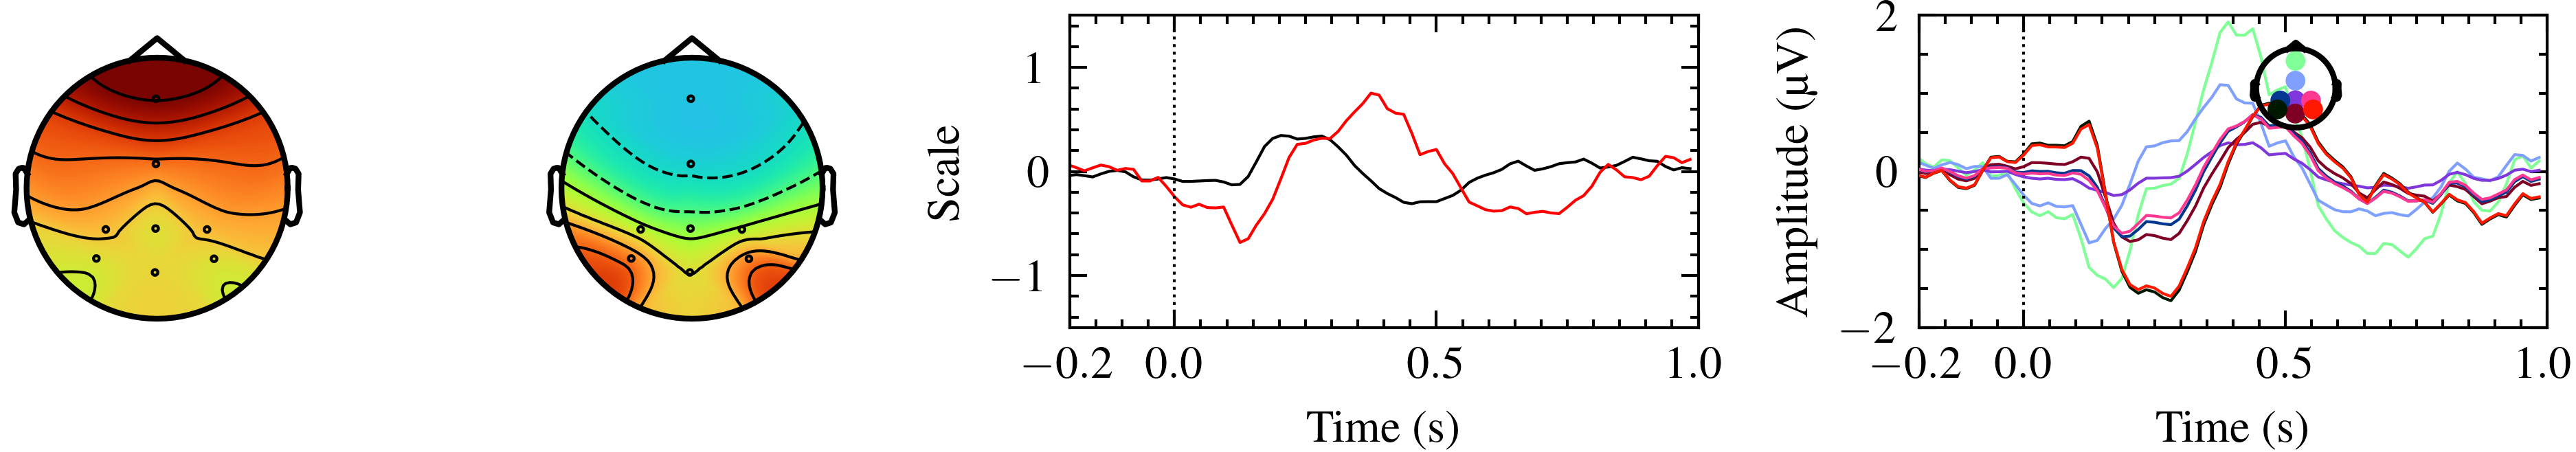
\includegraphics[width=\linewidth]{figure6a.png}
%	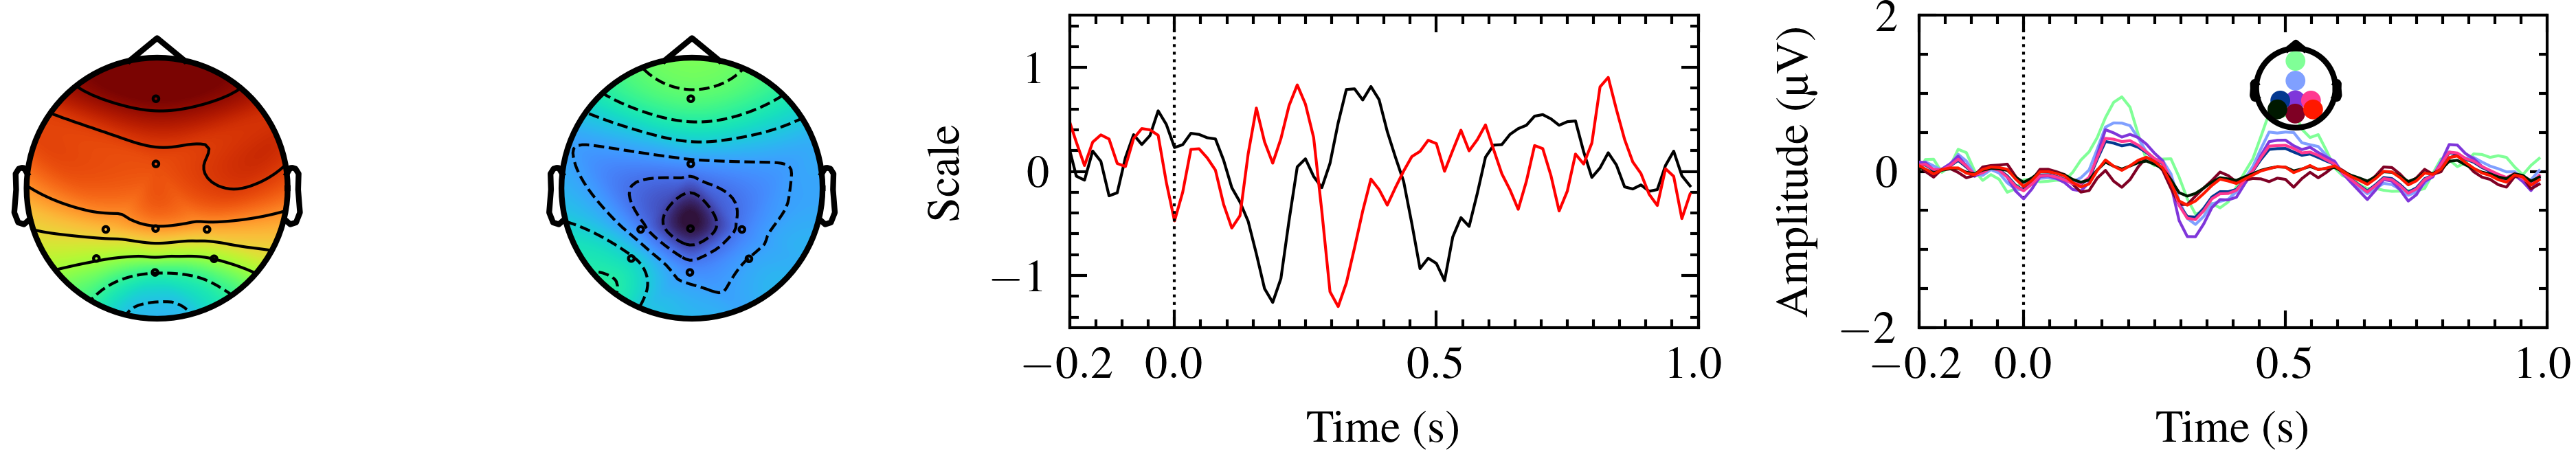
\includegraphics[width=\linewidth]{figure6b.png}
%  \caption[Extracted \acs{bttda} activation patterns.]{%
%    Spatial (left two columns) and temporal (middle column) activation patterns and
%		condition contrasts (right column) obtained after forward projection of the latent
%    features for 2 blocks of rank $(2,2)$ of \ac{bttda}
%    fit on the full dataset BNCI2014-008.
%    The separate blocks approximately model different \ac{erp}
%		components.}
%	\label{fig:forward}
%\end{figure*}
%Given informed or correctly tuned hyperparameters, this method could be used to
%e.g., separate \ac{erp} components or neural processes based on the task-related
%information in the class labels.


\subsection{Model selection and dimensionality}
\todo[inline]{replace by interpretation of new model selection procedure}

\Ac{bttda} trades in the rigid \ac{hoda} model for increased model complexity with more
hyperparameters to tune, which could open up a setting where performance can be
improved.
This shifts the focus of tensor discriminant analysis  from projection
optimization to model selection.
Despite favorable results in \ac{bci} decoding, the applications of the proposed
\ac{bttda} model are limited mainly by this model selection approach used
to determine the individual block ranks.
\todo[inline]{drop greedy}
While our proposed greedy model selection algorithm is a step in the right
direction, the high computational cost of setting hyperparameters through cross
validation can still hinder the portability of decoders relying on
\ac{bttda}.

Due to its heuristic nature, the greedy algorithm does not always result in the
set of ranks with the highest achievable performance.
In combination with the fact that the feature selection cutoff parameter was
fixed somewhat arbitrarily, it is clear that thorough
hyperparameter optimization could improve performance.
Furthermore, it is clear that our proposed model selection procedure does not
necessarily result in an optimal set of blocks that group coherent projections
within the same block, according to some desirable metric.
Examples of this are sparsity, pattern interpretability, minimal or maximal
between- or within-block feature correlation, decreasing discriminability, etc.
Finally, the completeness of the presented results is limited by the artificial
restriction in hyperparameter choice.
\todo[inline]{rewrite to controlled by $\theta$}
We imposed $(r_1=r_2=\ldots=r_k)$ to reduce the computational demand of
the performed experiments.
In a sense, this goes against the proposition of increased model flexibility.
It might well be that \ac{bttda} in some cases offers little added value over the
Tucker-structured \ac{hoda}, when both are given free choice of rank.
Future efforts should focus automated parameter setting methods, e.g., using sparsity
or information criteria such as the ones used in Block-Term Tensor
Regression~\cite{Faes2022}, or other statistical measures based on the model's
application.

Another limitation is that \ac{bttda} might yield a disproportionate
improvement for datasets with a low number of features relative to sample size,
while being less effective for datasets with more features.
This is reflected in our \ac{erp} results (low dimensionality vs.\ high number of
trials) compared to the \ac{mi} results (higher dimensionality due to third-order
tensorization vs.\ lower number of trials).
\todo[inline]{is this still the case?}
We expect a dimensionality limit beyond which the forward modeling step cannot
accurately regress from the low-dimensional latent tensors to the high-
dimensional original tensors, introducing
error in the input data for the next block, which can stack up over blocks.
Since the forward multilinear least squares problem is underdetermined, it is
prone to numerical instability, which calls for regularization of the forward
modeling procedure, but this would introduce another hyperparameter.
It should also be thoroughly investigated what the impact is of going beyond
second- and third-order cases to higher-order tensors, since this could have a
large impact on the model.
Other tensorization methods of the \ac{eeg} data, like time-lagged Hankel
tensors~\cite{Papy2005}, or tensors across subjects or sliding windows, etc.,
could also be of interest if they are appropriately chosen based on prior
knowledge of the dataset.

\section{Conclusion}

We have introduced \acf{bttda}, a novel,
tensor-based, supervised dimensionality reduction technique optimized for class
discriminability, which adheres to the block-term tensor structure.
\ac{bttda} is a generalization of \acf{hoda} and can also be
applied as a special sum-of-rank-one tensors PARAFACDA model.
The model is obtained by iteratively fitting \ac{hoda} in a deflation scheme,
leveraging a novel forward modeling step.

Via an accompanying heuristic model selection procedure, \ac{bci} decoders using
\ac{bttda} feature extraction can significantly outperform decoders based on
\ac{hoda} and reach state-of-the-art decoding performance on event-related potential
problems (second-order tensors) and scores on par with or higher than \ac{hoda} in motor
imagery problems (third-order tensors).
Moving from the rigid Tucker tensor structure of \ac{hoda} to the more flexible
and sparse block-term structure shifts the problem from finding optimally constrained
multilinear projections to model and feature selection.

Introducing a flexible block-term tensor model as the underlying structure
reformulates tensor discriminant analysis as a model selection
problem.
This allows performance to be traded off for model complexity and the number of
features, to find a setting that is more effective for decoding.
Because of its general implementation and minimal assumptions on data structure,
BTTDA can equally be applied to classification for other neuroimaging modalities
(MEG, ECoG, fNIRS, fMRI, EMG, etc.) or to tensor classification problems in other
fields.

\section*{Code availability}

The code of the proposed \ac{bttda} algorithm and the analyses performed in
this work are available at \url{https://github.com/arnevdk/bttda}.

\section*{Acknowledgements}
We thank the Flemish Supercomputer Center (VSC) and the High-Performance
Computing (HPC) center of the KU Leuven for allowing us to execute our
computational experiments on their systems.
We also wish to acknowledge dr.\ Axel Faes for his inspiration in
conceptualizing this work.

AVDK is funded by the special research fund of the KU Leuven (GPUDL/20/031).
MMVH is supported by research grants received from the European Union’s
Horizon Europe Marie Sklodowska-Curie Action program
(grant agreement No. 101118964), the European Union’s Horizon 2020 research and
innovation program (grant agreement No. 857375), the special research fund of
the KU Leuven (C24/18/098), the Belgian Fund for Scientific Research – Flanders
(G0A4118N, G0A4321N, G0C1522N), and the Hercules Foundation (AKUL 043).

The authors acknowledge the support by the RITMEA project co-financed by the
European Union with the European Regional Development Fund, the French state,
and the Hauts-de-France Region Council.

\printbibliography%
\clearpage%

\appendix
\setcounter{table}{0}
\renewcommand{\thetable}{A\arabic{table}}

\begin{table*}[ht]
	\footnotesize
	\begin{tabularx}{\linewidth}{@{}Xrrrrrrr@{}}
	\toprule
	Dataset                    & \# Sub.         & \# Chan. & \# Trials/class
	                           & \makecell{Epoch                                                                                          \\ len. (s)} & \makecell{S. freq.\\ (Hz)}
	                           & \# Sess.        & Ref.                                                                                   \\
	\midrule
	\textbf{\Ac{erp} datasets} &                 &          &                 &     &      &                   &                          \\
	BNCI2014-008               & 8               & 8        & 3500/700        & 1.0 & 256  & 1                 & \cite{Riccio2013}        \\
	BNCI2014-009               & 10              & 16       & 1440/288        & 0.8 & 256  & 3                 & \cite{Arico2014}         \\
	BNCI2015-003               & 10              & 8        & 1500/300        & 0.8 & 256  & 1                 & \cite{Guger2009}         \\
	BrainInvaders2012          & 25              & 16       & 640/128         & 1.0 & 128  & 2                 & \cite{VanVeen2019}       \\
	BrainInvaders2013a         & 24              & 16       & 3200/640        & 1.0 & 512  & 8 (sub. 1-7) or 1 & \cite{Vaineau2019}       \\
	BrainInvaders2014a         & 64              & 16       & 990/198         & 1.0 & 512  & up to 3           & \cite{Korczowski2019}    \\
	BrainInvaders2014b         & 38              & 32       & 200/40          & 1.0 & 512  & 3                 & \cite{Korczowski2019a}   \\
	BrainInvaders2015a         & 43              & 32       & 4131/825        & 1.0 & 512  & 3                 & \cite{Korczowski2019b}   \\
	BrainInvaders2015b         & 44              & 32       & 2160/480        & 1.0 & 512  & 1                 & \cite{Korczowski2019c}   \\
	Cattan2019-VR              & 21              & 16       & 600/120         & 1.0 & 512  & 2                 & \cite{Cattan2019}        \\
	%DemonsP300                 & 60              & 8                & 935/50          & 1.0  & 500  & 1                 & \cite{Goncharenko2020}   \\
	EPFLP300                   & 8               & 32       & 2753/551        & 1.0 & 2048 & 4                 & \cite{Hoffmann2008}      \\
	%ErpCore2021-ERN            & 40              & 30               & 400/400         & 1.0  & 1024 & 1                 & \cite{Kappenman2021}     \\
	%ErpCore2021-LRP            & 40              & 30               & 400/400         & 1.0  & 1024 & 1                 & \cite{Kappenman2021}     \\
	%ErpCore2021-MMN            & 40              & 30               & 800/200         & 1.0  & 1024 & 1                 & \cite{Kappenman2021}     \\
	%ErpCore2021-N170           & 40              & 30               & 240/80          & 1.0  & 1024 & 1                 & \cite{Kappenman2021}     \\
	%ErpCore2021-N2pc           & 40              & 30               & 160/160         & 1.0  & 1024 & 1                 & \cite{Kappenman2021}     \\
	%ErpCore2021-N400           & 40              & 30               & 60/60           & 1.0  & 1024 & 1                 & \cite{Kappenman2021}     \\
	%ErpCore2021-P3             & 40              & 30               & 160/40          & 1.0  & 1024 & 1                 & \cite{Kappenman2021}     \\
	Huebner2017                & 13              & 31       & 364/112         & 0.9 & 1000 & 3                 & \cite{Huebner2017}       \\
	Huebner2018                & 12              & 31       & 364/112         & 0.9 & 1000 & 3                 & \cite{Huebner2018}       \\
	Lee2019-ERP                & 54              & 62       & 6900/1380       & 1.0 & 1000 & 2                 & \cite{Lee2019}           \\
	Sosulski2019               & 13              & 31       & 7500/1500       & 1.2 & 1000 & 1                 & \cite{Sosulski2019}      \\
	\midrule
	\textbf{\Ac{mi} datasets}  &                 &          &                 &     &      &                   &                          \\
	AlexandreMotorImagery      & 8               & 16       & 20.0            & 3.0 & 512  & 1                 & \cite{Barachant2012}     \\
	%Beetl2021-A                & 4               & 63               &                 & 4.0  & 500  & 1                 & \cite{Wei2022}           \\
	%Beetl2021-B                & 2               & 32               &                 & 4.0  & 200  & 1                 & \cite{Wei2022}           \\
	BNCI2014-001               & 9               & 22       & 144.0           & 4.0 & 250  & 2                 & \cite{Tangermann2012}    \\
	%BNCI2014-002               & 14              & 15               & 80.0            & 5.0  & 512  & 1                 & \cite{Steyrl2016}        \\
	%BNCI2014-004               & 9               & 3                & 360.0           & 4.5  & 250  & 5                 & \cite{Leeb2007}          \\
	%BNCI2015-001               & 12              & 13               & 200.0           & 5.0  & 512  & 3                 & \cite{Faller2012}        \\
	%BNCI2015-004               & 9               & 30               & 80.0            & 7.0  & 256  & 2                 & \cite{Scherer2015}       \\
	%Cho2017                    & 52              & 64               & 100.0           & 3.0  & 512  & 1                 & \cite{Cho2017}           \\
	%Dreyer2023                 & 87              & 27               & 20.0            & 5.0  & 512  & 1                 & \cite{Pillette2021}      \\
	%Dreyer2023A                & 60              & 27               & 20.0            & 5.0  & 512  & 1                 & \cite{Pillette2021}      \\
	%Dreyer2023B                & 21              & 27               & 20.0            & 5.0  & 512  & 1                 & \cite{Pillette2021}      \\
	%Dreyer2023C                & 6               & 27               & 20.0            & 5.0  & 512  & 1                 & \cite{Pillette2021}      \\
	%GrosseWentrup2009          & 10              & 128              & 150.0           & 7.0  & 500  & 1                 & \cite{GrosseWentrup2009} \\
	%Lee2019-MI                 & 54              & 62               & 100.0           & 4.0  & 1000 & 2                 & \cite{Lee2019}           \\
	%Liu2024                    & 50              & 29               & 20.0            & 4.0  & 500  & 1                 & \cite{Liu2024}           \\
	%Ofner2017                  & 15              & 61               & 60.0            & 3.0  & 512  & 1                 & \cite{Ofner2017}         \\
	%	PhysionetMotorImagery      & 109             & 64       & 23.0            & 3.0 & 160  & 1                 & \cite{Goldberger2000}    \\
	Schirrmeister2017          & 14              & 128      & 120.0           & 4.0 & 500  & 1                 & \cite{Schirrmeister2017} \\
	%Shin2017A                  & 29              & 30               & 30.0            & 10.0 & 200  & 3                 & \cite{Shin2016}          \\
	%Shin2017B                  & 29              & 30               & 30.0            & 10.0 & 200  & 3                 & \cite{Shin2016}          \\
	%Stieger2021                & 62              & 64               & 450.0           & 3.0  & 1000 & 7 or 11           & \cite{Stieger2021}       \\
	Weibo2014                  & 10              & 60       & 80.0            & 4.0 & 200  & 1                 & \cite{Yi2014}            \\
	Zhou2016                   & 4               & 14       & 160.0           & 5.0 & 250  & 3                 & \cite{Zhou2016}          \\
	\bottomrule
\end{tabularx}

	\caption[MOABB datasets used for evaluation.]{MOABB datasets used for evaluation, with the number of
		subjects (\# Sub.), the number of EEG channels (\# Chan.), the number of
		classes (\# Class.), the number of trials or trials per class for ERP
		datasets (\# Trials), the epoch length (Epoch len.), the sampling
		frequency (S. freq.), the number of sessions per subject (\# Sess.) and the
		number of runs (\# Runs).
		Adapted from~\cite{Aristimunha2023}
		and~\cite{Chevallier2024}.}
	\label{tab:moabb}
\end{table*}

\pagebreak

\end{document}
